\فصل{تعاریف و مفاهیم اولیه}

پیش از مرور کارهای انجام شده در زمینه‌ی انتشار داده و حفظ حریم خصوصی و همچنین تشخیص فعالیت‌های کاربران در خانه های هوشمند نیاز است تا در ابتدا تعاریف و مفاهیمی پایه‌ای مورد نیاز ارائه گردد.

\section{مفاهیم پایه}

در حوزه خانه هوشمند و تشخیص فعالیت کاربران مفاهیم و اصطلاحات زیادی مطرح است که جهت شفاف‌سازی و ایجاد درک مشترک از مطالب ارائه شده، هر یک را به صورت دقیق تعریف می‌کنیم.

\begin{itemize}
\item \textbf{\پاورق{‌همبستگی}{Correlation}}: همبستگی، ارتباط بین دو یا چند \پاورق{‌موجودیت}{Entity} را نشان می‌دهد که به معنی تاثیرگذاری آن‌ها روی یکدیگر است \cite{x211}.
\item \textbf{\پاورق{‌زمینه}{Context}}: با توجه به تعریف \پاورق{‌هونگ}{Hong} و همکاران \cite{x212} و همچنین تعریف \پاورق{‌رودریگز}{Rodriguez} و همکاران \cite{x213}، زمینه به هرگونه اطلاعات که برای توصیف وضعیت یک موجودیت استفاده می‌شود گفته می‌شود. در این پژوهش از تعریف \پاورق{‌یسایی}{Yasaei} و همکاران \cite{x2147777} استفاده شده است. این تعریف بیان می‌کند که زمینه شرایطی است که سیستم در آن کار می‌کند و آن شرایط بر نتیجه سیستم تاثیر می‌گذارد.
\item \textbf{\پاورق{‌معناشناسی}{Semantics}}: شاخه‌ای از زبان‌شناسی و منطق است که تحلیل معنا و روابط بین کلمات را در خود دارد. زمانی که در سیستمی به اطلاعات معنا داده می‌شود به طوری که برای کاربران و رایانه‌ها قابل فهم و تعامل باشد، مجهز به ابزار معناشناسی است \cite{x213}.
\item \textbf{\پاورق{‌رخداد}{Event}}: داده دریافتی از حسگرها است که بیانگر حالت حسگر یا نقدار اندازه‌گیری شده توسط حسگر در لحظه‌ای از زمان است \cite{x3228}. 
\item \textbf{\پاورق{‌فعالیت}{Activity}}: مجموعه‌ای از رخدادها که نمایانگار تاثیرات یک فعالیت انسانی، مانند ظرف شستن یا مسواک زدن، بر روی حسگرهای نصب شده در محیط باشد \cite{xyz1}. 
\item \textbf{\پاورق{‌رفتار}{Behaviour}}: در حالی که دسته‌ای از پژوهش‌ها \cite{x3212, xyz2, xyz3} دو واژه فعالیت و رفتار را هم‌معنی دانسته‌اند؛ در این پژوهش از تعریف دسته دیگر \cite{xyz4, xyz5} استفاده شده است که رفتار را یک سطح بالاتر و به عنوان مجموعه‌ای از فعالیت‌ها می‌دانند.
\end{itemize}

\section{روش‌های داده‌محور، دانش‌محور و ترکیبی}\label{chapter:c22}

روش‌ها در هوش مصنوعی به سه دسته‌ی \پاورق{داده‌محور}{Data-driven}، \پاورق{دانش‌محور}{Knowledge-driven} و ترکیبی تقسیم می‌شوند \cite{x221,x222}:

\begin{itemize}
\item \textbf{روش‌های داده‌محور}: این روش‌ها به صورت خودکار و با استفاده از تکنیک‌های \پاورق{‌یادگیری ماشین}{Machine learning}، داده‌های جمع شده تا لحظه کنونی را تبدیل به مدل‌ می‌کنند. روش‌های داده محور در محیط‌های پویا کاربردی بوده و دقت بالایی دارند اما در صورتی که نیاز به دانش با در نظر گرفتن زمینه باشد دچار مشکل می‌شود. با توجه به این مشکل امکان استفاده مجدد یک موجودیت برای موجودیت دیگر وجود ندارد و برای هر موجودیت مدلی جدا برای آموزش نیاز است. همچنین داده زیادی برای آموزش مورد نیاز است که زمانی طول می‌کشد تا به بهره‌وری برسد که اصطلاحا \پاورق{‌شروع سرد}{Cold-start} نام دارد. توجه شود که بعضی فعالیت‌ها به ندرت انجام شده و این فعالیت‌های مشاهده نشده نقطه ضعف این روش هستند چرا که تا زمان عدم مشاهده‌ی این فعالیت‌ها، مدل‌سازی ناقص بوده و حتی با گذشت زمان زیادی از یادگیری مدل، نمی‌توان اطمینان از کامل بودن آن داشت.
\item \textbf{روش‌های دانش‌محور}: در این دسته از روش‌ها \پاورق{‌فرد خبره}{Expert} با دانش پیشین از حوزه، مدل را به صورت دستی ایجاد می‌کند. این روش زمینه را در نظر می‌گیرد و قابلیت استفاده مجدد دارد. همچنین این روش مشکل شروع سرد را ندارد زیرا نیاز به داده اولیه برای آموزش ندارد و با توجه به دانش فرد خبره به خودی خود کامل است اما نیاز است تا فرد خبره دانش کامل و عمیقی داشته باشد. عیب دیگر این روش ایستا بودن آن است که تغییرات فعالیت کاربران لحاظ نمی‌شود و نیاز است به صورت دستی به‌روز شوند.
\item \textbf{روش‌های ترکیبی}: این روش‌ها ‌از ترکیب روش‌های داده‌محور و دانش‌محور استفاده می‌کنند تا محدودیت و نقاط ضعف این روش‌ها را برطرف نمایند و از نقاط قوت آن‌ها بهره ببرند.
\end{itemize}

\section{هستی‌شناسی}

هستی‌شناسی نمایش \پاورق{‌صوری}{Formal} دانش توسط مجموعه‌ای از \پاورق{‌مفاهیم}{Concepts}، خصوصیات و محدودیتشان و همچنین روابط بین این مفاهیم است \cite{x231}. هستی‌شناسی (\پاورق{‌تی‌باکس}{Terminology box (TBox)}) به همراه مجموعه‌ای از \پاورق{‌نمونه‌ها}{Instances} (\پاورق{‌ای‌باکس}{Assertion box (ABox)}) پایگاه دانش را تشکیل می‌دهند. ای باکس شامل نمونه‌هایی از عناصر تعریف شده در تی‌باکس است (به همراه \پاورق{‌روابط}{Relations}).
هستی‌شناسی در حوزه‌های مختلف از جمله \پاورق{‌وب معنایی}{Semantic web}، \پاورق{‌موتورهای جستجو}{Search engines}، \پاورق{‌تجارت الکترونیکی}{Electronic commerce}، \پاورق{‌پردازش زبان‌های طبیعی}{Natural Language Processing}، \پاورق{‌مهندسی دانش}{Knowledge engineering}، \پاورق{‌بازیابی اطلاعات}{Data recovery} و اینترنت اشیاء کاربرد دارد. از مزایای استفاده از هستی‌شناسی می‌توان به موارد زیر اشاره نمود:

\begin{itemize}
\item ایجاد یک فهم مشترک از ساختار اطلاعات
\item امکان استفاده مجدد
\item امکان تحلیل روی دانش
\end{itemize}

به طور کلی هستی‌شناسی شامل اجزای اصلی زیر است:

\begin{itemize}
\item \textbf{مفاهیم}: مجموعه‌ یا کلاسی از موجودیت‌ها یا چیزهایی که درون یک حوزه وجود دارد.
\item \textbf{روابط}: روابط یا ارتباطات برای بیان تعاملات بین مفاهیم و یا معین کردن ویژگی‌‌های یک مفهوم به کار می‌‌رود و در هستی‌شناسی دو نوع رابطه بین موجودیت‌ها وجود دارد. ارتباط رده‌بندی که سازماندهی مفاهیم در یک ساختار سلسله مراتبی را نشان می‌‌دهد مانند ارث‌بری کلاس‌ها در شیءگرایی و ارتباطات پیوندی که ارتباط مفاهیمی را با یکدیگر به نمایش می‌‌گذارد که در یک ساختار سلسله مراتبی به هم مرتبط نمی‌‌باشند.
\item \textbf{نمونه‌ها}: اعضا یا نمونه‌ها همان چیزهایی هستند که توسط یک مفهوم معرفی می‌شوند مثلاً در حوزه مدارس، مدرسه‌‌ای با نام «مدرسه الف» عضوی از مفهوم مدرسه است. توجه باید کرد که یک هستی‌شناسی به خودی خود نمونه‌ای ندارد و صرفاً عبارت است از طراحی ساختاری از مفاهیم یک حوزه که ترکیب آن با اعضاء و نمونه‌ها، پایگاه دانش آن حوزه را ایجاد می‌‌نماید.
\item \textbf{\پاورق{‌قواعد}{Rules}}: قاعده‌‌ها برای مقید کردن مقادیر برای کلاس‌ها یا ویژگی‌‌ها مورد استفاده قرار می‌‌گیرند. مثلاً می‌توان گفت سن یک انسان باید بیشتر از ۰ و کمتر از ۱۲۰ باشد.
\end{itemize}

تا کنون زبان‌های هستی‌شناسی زیادی توسعه یافته‌اند. این زبان‌ها عموما بر پایه زبان \پاورق{‌\lr{XML}}{eXtensible Markup Language} \cite{x233} هستند که قابلیت تفسیر و سادگی معناشناسی برای ماشین را دارند. از این زبان‌ها می‌توان به \پاورق{‌\lr{RDF}}{Resource Description Framework} و \lr{RDF Schema} \cite{x234}، \پاورق{‌\lr{OIL}}{Ontology Inference Layer} + \پاورق{‌\lr{DAML}}{DARPA Agent Markup Language} \cite{x235}، \lr{OWL} \cite{x236} و \lr{OWL2} \cite{x236Z} اشاره کرد. یکی از پرکاربردترین آن‌ها \پاورق{‌\lr{OWL}}{Ontology Web Language} است که روی \lr{RDF} و \lr{OIL} + \lr{DAML} توسعه یافته است و قدرت بیان بالایی دارد. \lr{OWL} دارای سه زیرزبان \lr{OWL-Lite} ،\lr{OWL-Full} و \lr{OWL-DL} است و زبان توصیف قواعد \پاورق{‌\lr{SWRL}}{Semantic Web Rule Language} \cite{x237} امکان نوشتن قواعد را به \lr{OWL-DL} اضافه کرده تا قدرت بیان آن را افزایش دهد.

\section{قوانین انجمنی‌}\label{chapter:c24}

\پاورق{‌قوانین انجمنی}{Associative rules} در داده‌کاوی و یادگیری ماشین به دنبال کشف ارتباطات و تعاملات بین عناصر در مجموعه داده هستند \cite{x241}. این نوع ارتباط‌ها به طور معمول بر روی داده‌های تراکنشی مانند فروش‌های خرده‌فروشی یا خرید‌های آنلاین کاربرد دارند. این قوانین دارای دو تعریف اساسی \پاورق{‌پشتیبانی}{Support} و \پاورق{‌اطمینان}{Confidence} هستند:

\begin{itemize}
\item \textbf{پشتیبانی}: پشتیبانی، فرکانس درست بودن یک قانون در یک مجموعه داده معین را اندازه گیری می‌کند و نشان دهنده نسبت تراکنش هایی است که هم موارد موجود در مقدمه و هم موارد موجود در نتیجه قانون را شامل می شود و کمک می‌کند تا کاربرد یک قانون مشخص شود، و از آن برای کشف قوانین رایج یا مکرر در مجموعه داده استفاده می‌شود. 
\item \textbf{اطمینان}: اطمینان، احتمال مشروط بودن موارد موجود در نتیجه یک قانون را با توجه به اینکه موارد موجود در مقدمه درست هستند، اندازه گیری می کند. در واقع قابلیت اطمینان یک قانون را نشان می‌دهد و اینکه هر چند وقت یک‌بار حضور عناصر را در نتیجه به درستی پیش‌بینی می‌کند، در حالی که عناصر مقدمه وجود دارند.
\end{itemize}

قوانین انجمنی برای کشف ارتباطات مفهومی و معنادار بین عناصر در مجموعه داده استفاده می‌شوند و در مواردی مانند تجزیه و تحلیل سبد خرید، سیستم‌های پیشنهادی، و اتخاذ تصمیمات در داده‌کاوی و تحلیل داده مورد استفاده قرار می‌گیرند.

\section{زیست‌بوم خانه‌های هوشمند‌}

با استفاده از امکانات خانه‌های هوشمند کاربران می‌توانند دستگاه‌های اینترنت اشیاء را از راه دور کنترل کنند. ضمن این که کارهای مختلفی نیز می‌تواند به صورت خودکار برای سهولت زندگی انسان در این زیرساخت انجام شود. معماری رایج خانه‌های هوشمند در شکل \ref{fig:f21} نشان داده شده است.

\begin{figure}[htp]
\centerline{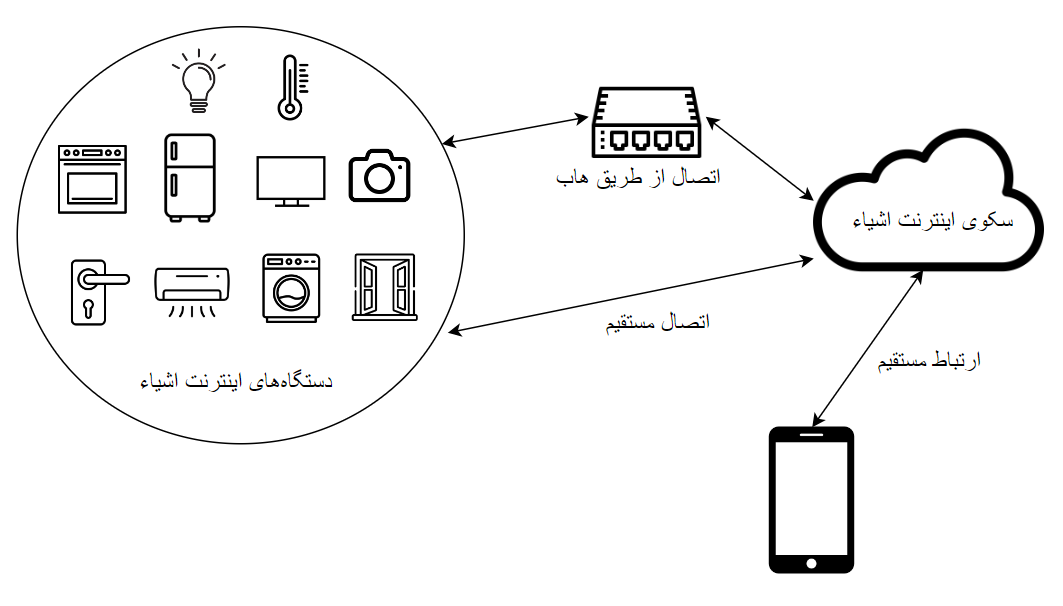
\includegraphics[width=0.8\textwidth]{figs/f21.png}}
\caption[معماری رایج خانه‌های هوشمند]{معماری رایج خانه‌های هوشمند \cite{x251}}
\label{fig:f21}
\end{figure}

خانه های هوشمند شامل اجزای زیر هستند:

\begin{itemize}
\item \textbf{دستگاه‌های اینترنت اشیاء}: دستگاه‌های اینترنت اشیاء شامل حسگر و یا \پاورق{‌عملگرهایی}{Actuators} هستند که حسگرها خصوصیتی را اندازه‌گیری می‌کنند و عملگرها کنشی را انجام می‌دهند. به عنوان مثال حسگر نور، نور محیط را اندازه‌گیری کرده و در صورت بالا بودن شدت نور، عملگر نور محیط را کم می‌کند. عملکرد یک عملگر می‌تواند به صورت خودکار یا به صورت دستی انجام شود.
دستگاه‌ها در خانه‌ هوشمند به دو دسته تقسیم می‌شوند \cite{x252}:
\begin{itemize}
\item \textbf{دستگاه‌های متصل به \پاورق{‌ابر}{Cloud}}: این دستگاه‌ها با فناوری \پاورق{‌وای‌فای}{Wi-Fi} با زیرساخت ابری ارتباط برقرار می‌کنند. استفاده از وای‌فای به دلیل مصرف زیاد انرژی قابل استفاده در تمامی دستگاه‌ها نیست و اکثر دستگاه‌ها از فناوری دیگری بهره می‌برند.
\item \textbf{دستگاه‌های متصل به \پاورق{‌هاب}{Hub}}: این دستگاه‌ها دارای فناوری وای‌فای نبوده و ارتباطشان با زیرساخت ابری از طریق فناوری‌هایی با مصرف انرژی کم است. از این فناوری‌ها می‌توان به \پاورق{‌زی‌ویو}{Z-Wave} و \پاورق{‌زیگ‌بی}{Zigbee} اشاره کرد. این دستگاه‌ها از طریق هاب با زیرساخت ابری ارتباط برقرار می‌کنند.
\end{itemize}

دستگاه‌های خانه هوشمند ممکن است از یک یا هر دو نوع ذکر شده پشتیبانی کنند.

\item \textbf{هاب}: هاب دستگاهی است که به امواج بی‌سیم با برد کم مانند زی‌ویو، زیگ‌بی و وای‌فای مجهز است. دستگاه‌های اینترنت اشیاء از طریق هاب با یکدیگر و زیرساخت ابری ارتباط برقرار می‌کنند.
\item \textbf{زیرساخت ابری}: زیرساخت ابری پردازش‌های مربوطه را روی داده‌های دریافتی انجام می‌دهد و امکان خودکارسازی امور را با استفاده از نرم‌افزارهای اینترنت اشیاء فراهم میکند.
\item \textbf{نرم‌افزار تلفن همراه}: نرم‌افزار مدیریتی دستگاه‌ها و هاب که به کاربر این امکان را می‌دهد که تمامی اجزا را کنترل کند.

\end{itemize}

\section{سکوهای اینترنت اشیاء‌}

سکوهای اینترنت اشیاء امکان خودکارسازی ارتباطات بین دستگاه‌های اینترنت اشیاء با یکدیگر را فراهم می‌کند. این سکوها عموما از مدل رویداد-کنش استفاده می‌کنند. برنامه‌های اینترنت اشیاء می‌توانند روی این سکوها توسعه یافته و قوانین خودکارسازی خود را پیاده کنند. یعنی زمانی که رویدادی مشخص رخ دهد، سکو دستور مربوط به آن رخداد را ارسال می‌کند.
امروزه سکوهای اینترنت اشیاء زیادی وجود دارد که می‌توان به \پاورق{‌\lr{IFTTT}}{If This Then That} \cite{x261}، \پاورق{‌اسمارت‌تینگز}{SmartThings} \cite{x262}، \پاورق{‌اپن‌هاب‌}{OpenHAB} \cite{x263}، \پاورق{‌زپیر‌}{Zapier} \cite{x264}، \پاورق{‌اپل هوم‌کیت‌}{Apple home kit} \cite{x265} و \پاورق{‌مایکروسافت پاور اتومیت}{Microsoft power automate} \cite{x266} اشاره کرد. این سکوها از نظر زبان برنامه‌نویسی و معماری تفاوت دارند و به طور کلی همانطور که در بخش \ref{chapter:c24} اشاره شد به دو دسته ابرمحور و هاب‌محور تقسیم می‌شوند \cite{x267}. در سکوهای ابر‌محور مثل اسمارت‌تینگز که رایج‌تر هستند برنامه‌های اینترنت اشیاء روی زیرساخت ابری و در سکوهای هاب‌محور مثل اپل هوم‌کیت برنامه‌ها روی هاب اجرا می‌شوند. 
